\documentclass[10pt,twocolumn,letterpaper]{article}

%%%%%%%%% PAPER TYPE  - PLEASE UPDATE FOR FINAL VERSION
% \usepackage[review]{cvpr}      % To produce the REVIEW version
\usepackage{cvpr}              % To produce the CAMERA-READY version
%\usepackage[pagenumbers]{cvpr} % To force page numbers, e.g. for an arXiv version

% Include other packages here, before hyperref.
\usepackage{graphicx}
\usepackage{amsmath}
\usepackage{amssymb}
\usepackage{booktabs}
\usepackage[shortlabels]{enumitem}
\usepackage{color}

% It is strongly recommended to use hyperref, especially for the review version.
% hyperref with option pagebackref eases the reviewers' job.
% Please disable hyperref *only* if you encounter grave issues, e.g. with the
% file validation for the camera-ready version.
%
% If you comment hyperref and then uncomment it, you should delete
% ReviewTempalte.aux before re-running LaTeX.
% (Or just hit 'q' on the first LaTeX run, let it finish, and you
%  should be clear).
\usepackage[pagebackref,breaklinks,colorlinks]{hyperref}


% Support for easy cross-referencing
\usepackage[capitalize]{cleveref}
\crefname{section}{Sec.}{Secs.}
\Crefname{section}{Section}{Sections}
\Crefname{table}{Table}{Tables}
\crefname{table}{Tab.}{Tabs.}


%%%%%%%%% PAPER ID  - PLEASE UPDATE
\def\cvprPaperID{*****} % *** Enter the CVPR Paper ID here
\def\confName{CVPR}
\def\confYear{2025}
\newcommand{\add}[1]{{\color{blue}#1}}
\usepackage{tikz}
\usetikzlibrary{positioning}  % 用于节点定位
\usepackage{xcolor}  % 提供更多颜色选项

\begin{document}
	
	%%%%%%%%% TITLE - PLEASE UPDATE
	\title{NTIRE 2025 Efficient Burst HDR and Restoration\\A Hierarchical Fourier-based Transformer for Burst HDR and Restoration}
	
	% \author{
		% Sangmin Lee \hspace{2cm} Eunpil Park \hspace{2cm} Hyunhee Park\\
		% Samsung\\
		% Suwon, South Korea\\
		% {\tt\small \{sanggmin.lee, ep.park, inextg.park\}@samsung.com}
		% % For a paper whose authors are all at the same institution,
		% % omit the following lines up until the closing ``}''.
	% % Additional authors and addresses can be added with ``\and'',
	% % just like the second author.
	% % To save space, use either the email address or home page, not both
	% % \and
	% % Eunpil Park \\
	% % Samsung\\
	% % Suwon, Samsung\\
	% % {\tt\small ep.park@samsung.com}
	% }


% \maketitle



\author{Ruixuan Jiang\\
	USTC\\
	Anhui,China\\
	{\tt\small rxjiang21@gmail.com}
	\and
	Senyan Xu\\
	USTC\\
	Anhui,China\\
	{\tt\small syxu@mail.ustc.edu.cn}
	% For a paper whose authors are all at the same institution,
	% omit the following lines up until the closing ``''.
% Additional authors and addresses can be added with ``\and'',
% just like the second author.
% To save space, use either the email address or home page, not both
\and
Xingbo Wang\\
USTC\\
Anhui,China\\
{\tt\small wxb864557356@mail.ustc.edu.cn}
}
\maketitle

\section{Team Details}
\textbf{Team Name:} E\_Group\\
\textbf{Team Members:}
\begin{itemize}
	\item Senyan Xu
	\item Xingbo Wang
	\item Ruixuan Jiang 
\end{itemize}
\
\textbf{Username:} accept\\
\textbf{File Name:} 	c256.zip\\
\textbf{PSNR:} 40.64\\
\textbf{Best Score:} SFHformer2\_ft6\_5e-6\_batch2\_4000.zip (03/12/2025 12:10:26) PSNR: 41.73(development phase)\\
\textbf{Code Link:} \url{https://github.com/Levi202309/NTIRE-2025-Burst}

\section{Method Details}
Our proposed model utilizes the SFHFormer \cite{FFT1} block, which consists of a hierarchical encoder-decoder structure composed of five stages. The structure includes a two-scale encoder (stage-1 and stage-2), a bottleneck (stage-3), and a two-scale decoder (stage-4 and stage-5). The core components of our SFHFormer block are: (a) Local Global Perception Mixer (LGPM) and (b) Multi-kernel ConvFFN (MCFN). The LGPM is designed to capture both local and global feature representations, while the MCFN enhances the feature transformation capabilities through multiple kernel convolutions.

\subsection{figure of the model}
See the figure on the right.
\begin{figure}[!htb]
	\centering
	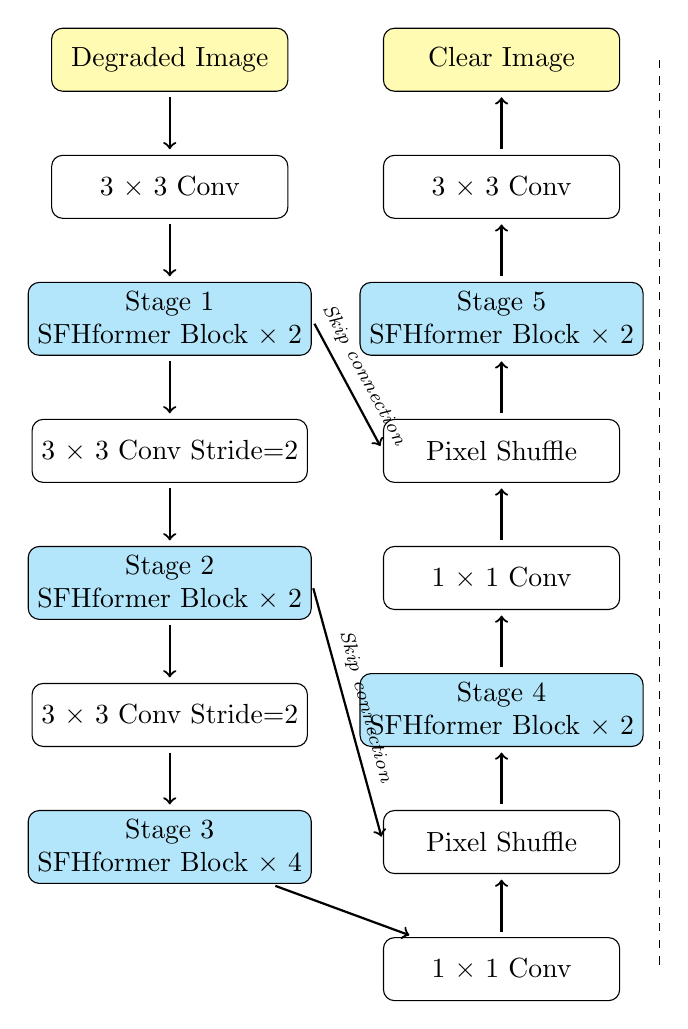
\begin{tikzpicture}[
		node distance=0.8cm,  % 减小节点间距
		box/.style={rectangle, draw, rounded corners, minimum width=3cm, minimum height=0.8cm, text centered},  % 减小宽度
		sfibox/.style={rectangle, draw, fill=cyan!30, rounded corners, minimum width=3cm, minimum height=0.8cm, text centered, align=center},  % 减小宽度
		arrow/.style={->, thick, shorten >=2pt, shorten <=2pt}  % 使用shorten选项缩短箭头长度
		]
		% 左侧流程 - 从上到下
		\node[box, fill=yellow!30] (degraded) {Degraded Image};
		\node[box, below=of degraded] (conv1) {3 $\times$ 3 Conv};
		\node[sfibox, below=of conv1] (stage1) {Stage 1\\SFHformer Block $\times$ 2};
		\node[box, below=of stage1] (conv2) {3 $\times$ 3 Conv Stride=2};
		\node[sfibox, below=of conv2] (stage2) {Stage 2\\SFHformer Block $\times$ 2};
		\node[box, below=of stage2] (conv3) {3 $\times$ 3 Conv Stride=2};
		% 下方矩形,现在宽度和其他stage一致
		\node[sfibox, below=of conv3] (stage3) {Stage 3\\SFHformer Block $\times$ 4};
		% 右侧流程 - 从下往上
		\node[box, fill=yellow!30, right=1.2cm of degraded] (clear) {Clear Image};  % 减小水平间距
		\node[box, below=of clear] (conv4) {3 $\times$ 3 Conv};
		\node[sfibox, below=of conv4] (stage5) {Stage 5\\SFHformer Block $\times$ 2};
		\node[box, below=of stage5] (shuffle1) {Pixel Shuffle};
		\node[box, below=of shuffle1] (conv5) {1 $\times$ 1 Conv};
		\node[sfibox, below=of conv5] (stage4) {Stage 4\\SFHformer Block $\times$ 2};
		\node[box, below=of stage4] (shuffle2) {Pixel Shuffle};
		\node[box, below=of shuffle2] (conv6) {1 $\times$ 1 Conv};
		% 连接箭头 - 严格按照图片,使用相同的arrow样式确保粗细一致
		\draw[arrow] (degraded) -- (conv1);
		\draw[arrow] (conv1) -- (stage1);
		\draw[arrow] (stage1) -- (conv2);
		\draw[arrow] (conv2) -- (stage2);
		\draw[arrow] (stage2) -- (conv3);
		\draw[arrow] (conv3) -- (stage3);
		% 右侧箭头方向从下往上,使用相同的arrow样式确保粗细一致
		\draw[arrow] (stage3) -- (conv6);
		\draw[arrow] (conv6) -- (shuffle2);
		\draw[arrow] (shuffle2) -- (stage4);
		\draw[arrow] (stage4) -- (conv5);
		\draw[arrow] (conv5) -- (shuffle1);
		\draw[arrow] (shuffle1) -- (stage5);
		\draw[arrow] (stage5) -- (conv4);
		\draw[arrow] (conv4) -- (clear);
		% Skip连接 - 箭头从左到右,使用较短的路径和相同的arrow样式
		\draw[arrow] (stage1.east) -- (shuffle1.west) node[midway, above, sloped] {\scriptsize \textit{Skip connection}};
		\draw[arrow] (stage2.east) -- (shuffle2.west) node[midway, above, sloped] {\scriptsize \textit{Skip connection}};
		% 垂直虚线,在最右侧
		\draw[dashed] ([xshift=0.5cm]clear.east) -- ([xshift=0.5cm]conv6.east);
	\end{tikzpicture}
	\caption{Model Architecture}
	\label{fig:model_architecture}
\end{figure}


\subsection{Training Strategy}
AdamW optimizer with $\beta_1$ and $\beta_2$ equal to 0.9 and 0.999 is used to train SFHformer. The initial learning rate is set as $7.5 \times 10^{-4}$. We adopt the cosine annealing strategy to train the models, where the learning rate gradually decreases from the initial learning rate to $5 \times 10^{-6}$. All experiments are implemented by PyTorch 1.11.0 with two NVIDIA 4090 GPUs. We used batch-size of 2 and crop-size of 256.

\subsection{Experimental Results}
The highest metric achieved in the testing phase was 40.59 PSNR.


\begin{thebibliography}{00}
	
	\bibitem[Jiang et al.(2024)]{FFT1} %item1
	Jiang, X., Zhang, X., Gao, N., and Deng, Y. (2024). "When Fast Fourier Transform Meets Transformer for Image Restoration." European Conference on Computer Vision: 381-402. 
	%item2,...,itemn
\end{thebibliography}


\end{document}